%\section{Used Datasets}
%\begin{figure}
%\begin{minipage}{0.4\textwidth}
%    The datasets used for this project, inlcuding three main sets of data, make up the informations for a total of 8 features.
%    Since it will be the goal to predict COVID 19 cases, the data must contain confirmed cases on the geological smallets possible scale, for that if only countries are compared
%    the data will be reduced to approximatly 150 entries. For this project the data will come from the johns hopkins university which provides a well tracked essamble of confrimed corona cases on a city scale. 
%\end{minipage}
%    \begin{minipage}{0.59\textwidth}
%        \centering
%        \captionsetup{width=0.9\linewidth}
%        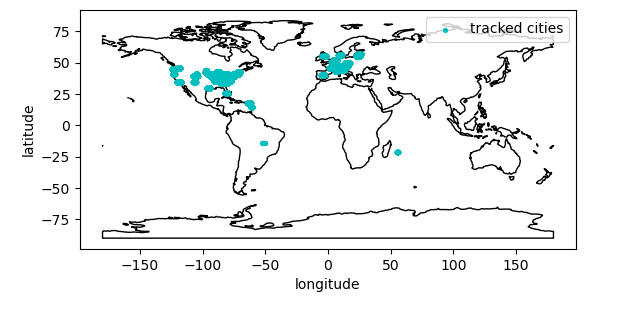
\includegraphics[width = 1\textwidth]{images/worldmap.png}
%        \caption{Shown is a schematic overview of the cities used to predict confimred corona cases using geopandas \cite{geopandas}.}
%    \end{minipage}
%\end{figure}
%\noindent
%Thus an unproccesed amount of approximatly 20000 cities, coded through latitude and longitude, with the features of interest are obtained.
%To collect worldwide weather data, again coded through latitude and longitude, the opensource platform \enquote{Metostat} \cite{metostat} will bee used. They provide a vast amount of features from which the 
%project will use the air pressure, avarage -, maximal -and minimal-temperature of each day. In a first step of merging both sets will be transformed to a \enquote{GeoPandasDataFrame}\cite{geopandas}
%which creates a new \enquote{Geometry} feature, containg botch longitude and latitude. With a choosen margin, in geopandas this is called \enquote{buffer}, the entries will be joined
%with its representing counterpart that is close i.e. in the margin of the first called buffer.  For this a buffer of $0.005$ has been choosen to allow some deviation since the geological datapoints of the combined sets might not be taken at  
%the exact same location.
%\begin{figure}
%    \centering
%    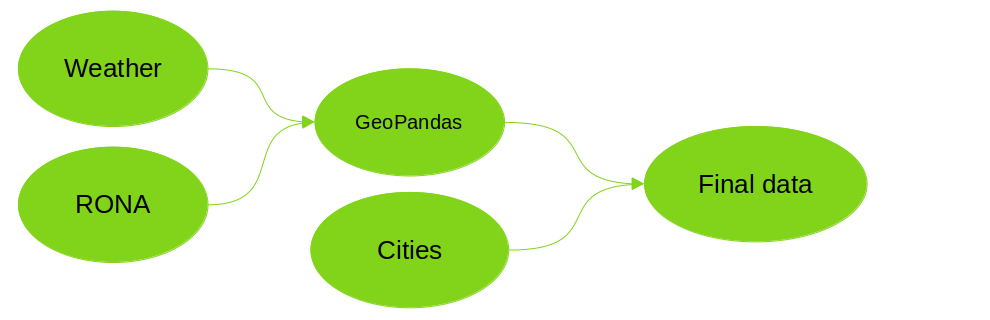
\includegraphics[width = 0.7\textwidth]{images/data_graph.png}
%    \caption{Shown is a schematic overview on how three different Dataset are used to form one final set with the desired features.}
%\end{figure}
%The final Datafram will inlcude the features: confirmed cases, minimal Temperature, maximal Temperature, average Temperature, air pressure, date and population. Note that the date will be transformed into 
%seconds, then divided by $10^{-8}$ rather than days months and years. \\
%\begin{figure}[H]
%    \centering
%    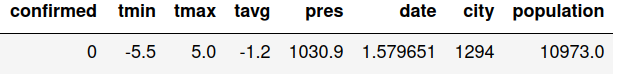
\includegraphics[width = 0.8\textwidth]{images/data_example.png}
%    \caption{Exampletory slice of the dataframe used to predict confirmed CONVID cases.}
%\end{figure}
%The scatter between the different features, including confirmed cases, can be seen in \ref{fig:scatter}.
%An obvious linear correlation between \enquote{T\_min}, \enquote{T\_max} and \enquote{T\_avg} can be seen 
%yet also an almost exponential growth in the confirmed-date cell.
%\begin{figure}[H]
%    \centering
%    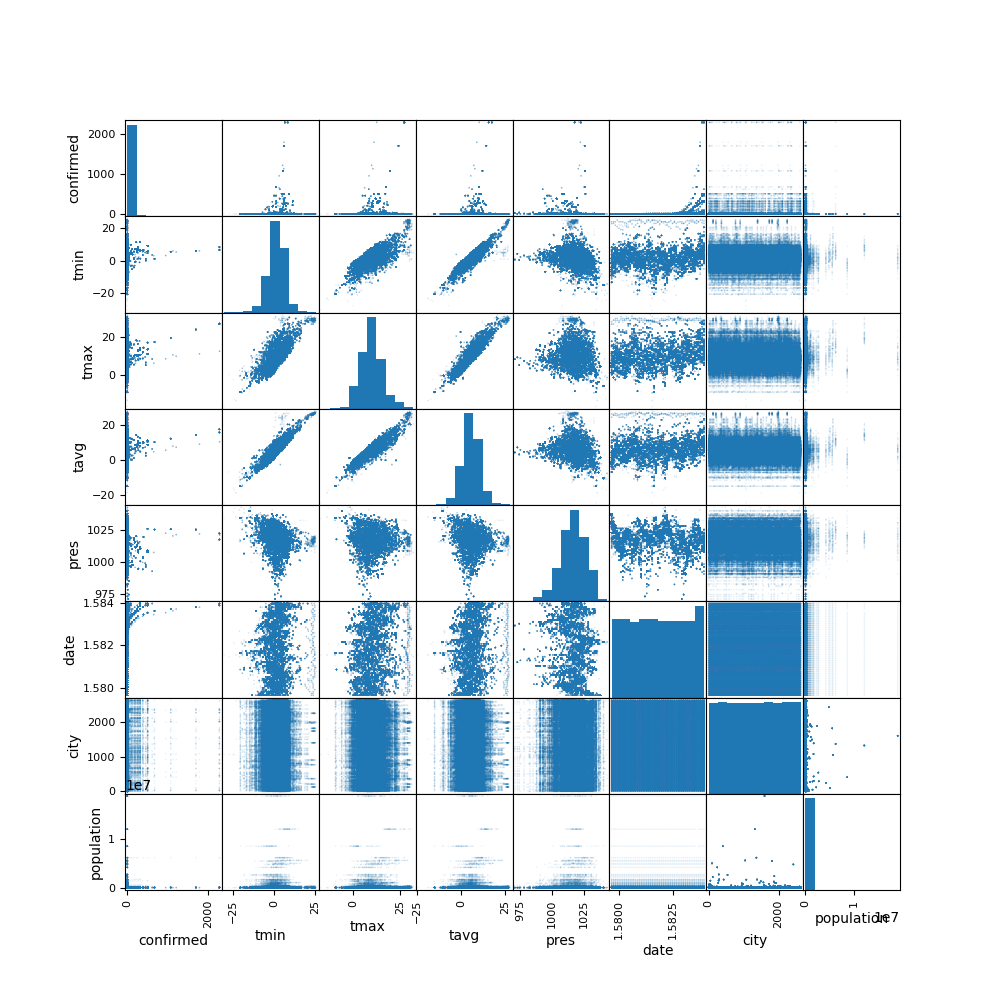
\includegraphics[width = 0.9\textwidth]{images/scatter.png}
%    \caption{This graphic shows a scatter matrix of a dataset that carries several features related to both weather and COVID confirmed cases.}
%\end{figure}


\section{Used Datasets}
\begin{figure}
\begin{minipage}{0.4\textwidth}
    %The datasets used for this project, inlcuding three main sets of data, make up the informations for a total of 8 features.
    %Since it will be the goal to predict COVID 19 cases, the data must contain confirmed cases on the geological smallets possible scale, for that if only countries are compared
    %the data will be reduced to approximatly 150 entries. For this project the data will come from the johns hopkins university which provides a well tracked essamble of confrimed corona cases on a city scale. 
    The datasets used for this project include three main sets of data, providing information on a total of 8 features. Since the primary goal is to predict COVID-19 cases, the data must contain confirmed cases on the smallest possible geographical scale. Therefore, if only countries are compared, the data will be reduced to approximately 150 entries. For this project, the data will come from Johns Hopkins University, which provides a well-tracked ensemble of confirmed corona cases on a city scale.
\end{minipage}
    \begin{minipage}{0.59\textwidth}
        \centering
        \captionsetup{width=0.9\linewidth}
        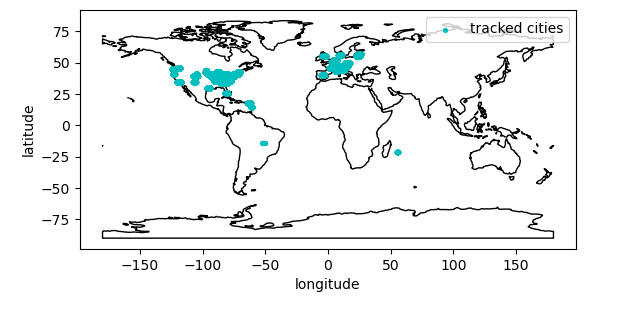
\includegraphics[width = 1\textwidth]{images/worldmap.png}
        \caption{Shown is a schematic overview of the cities used to predict confirmed corona cases using GeoPandas \cite{geopandas}.}
    \end{minipage}
\end{figure}
\noindent
%Thus an unproccesed amount of approximatly 20000 cities, coded through latitude and longitude, with the features of interest are obtained.
%To collect worldwide weather data, again coded through latitude and longitude, the opensource platform \enquote{Metostat} \cite{metostat} will bee used. They provide a vast amount of features from which the 
%project will use the air pressure, avarage -, maximal -and minimal-temperature of each day. In a first step of merging both sets will be transformed to a \enquote{GeoPandasDataFrame}\cite{geopandas}
%which creates a new \enquote{Geometry} feature, containg botch longitude and latitude. With a choosen margin, in geopandas this is called \enquote{buffer}, the entries will be joined
%with its representing counterpart that is close i.e. in the margin of the first called buffer.  For this a buffer of $0.005$ has been choosen to allow some deviation since the geological datapoints of the combined sets might not be taken at  
%the exact same location.
Thus, an unprocessed amount of approximately 20,000 cities, coded through latitude and longitude, with the features of interest, is obtained. To collect worldwide weather data, again coded through latitude and longitude, the open-source platform \enquote{Metostat} \cite{metostat} will be used. They provide a vast amount of features, from which the project will use the air pressure, average, maximal, and minimal temperatures of each day. In a first step, both sets will be transformed into a \enquote{GeoPandasDataFrame}\cite{geopandas}, which creates a new \enquote{Geometry} feature containing both longitude and latitude. With a chosen margin, in GeoPandas, this is called \enquote{buffer}, the entries will be joined with their representing counterparts that are close, i.e., within the margin of the first called buffer. For this, a buffer of $0.005$ has been chosen to allow some deviation since the geological data points of the combined sets might not be taken at the exact same location.
\begin{figure}
    \centering
    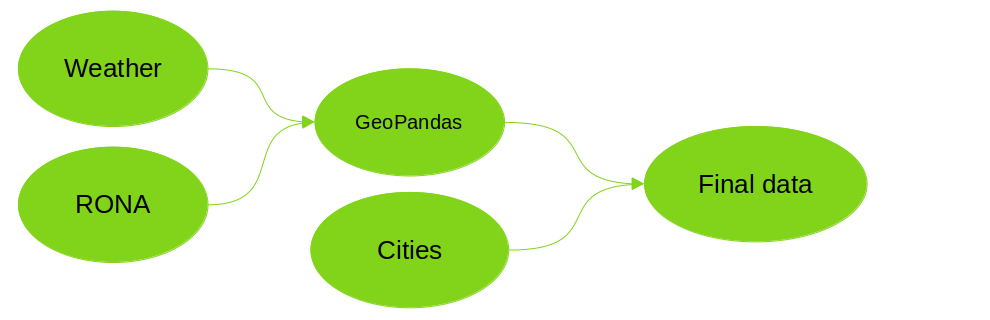
\includegraphics[width = 0.7\textwidth]{images/data_graph.png}
    \caption{Shown is a schematic overview of how three different datasets are used to form one final set with the desired features.}
\end{figure}
%The final Datafram will inlcude the features: confirmed cases, minimal Temperature, maximal Temperature, average Temperature, air pressure, date and population. Note that the date will be transformed into 
%seconds, then divided by $10^{-8}$ rather than days months and years. \\
The final DataFrame will include the features: confirmed cases, minimal temperature, maximal temperature, average temperature, air pressure, date, and population. Note that the date will be transformed into seconds, then divided by $10^{-8}$ rather than days, months, and years.
\begin{figure}[H]
    \centering
    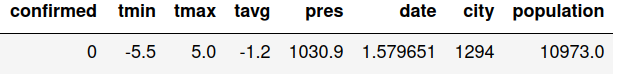
\includegraphics[width = 0.8\textwidth]{images/data_example.png}
    \caption{Exemplatory slice of the DataFrame used to predict confirmed COVID cases.}
\end{figure}
%The scatter between the different features, including confirmed cases, can be seen in \ref{fig:scatter}.
%An obvious linear correlation between \enquote{T\_min}, \enquote{T\_max} and \enquote{T\_avg} can be seen 
%yet also an almost exponential growth in the confirmed-date cell.
\noindent
The scatterplot between the different features, including confirmed cases, can be seen in Figure \ref{fig:scatter}.
An obvious linear correlation between \enquote{T\_min}, \enquote{T\_max}, and \enquote{T\_avg} can be observed.
Furthermore, there is an almost exponential growth in the confirmed cases over time.
\begin{figure}[H]
    \centering
    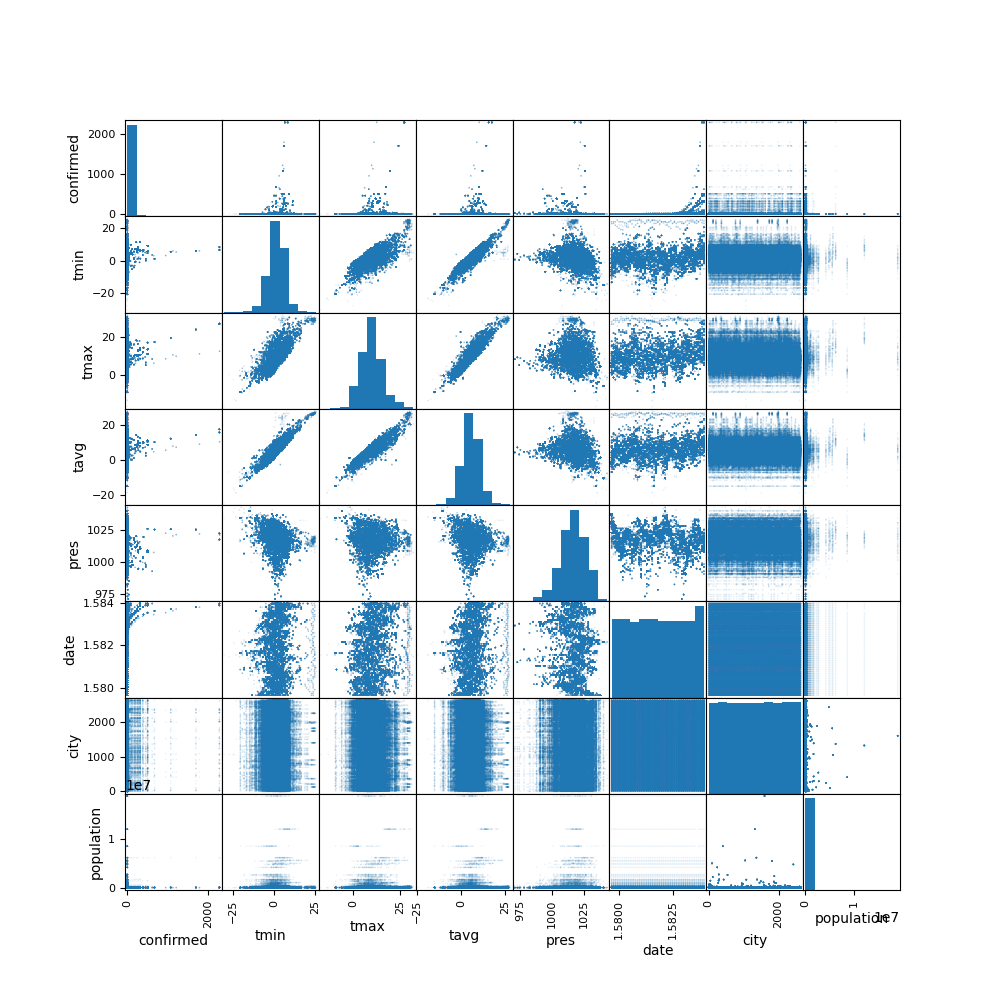
\includegraphics[width = 0.9\textwidth]{images/scatter.png}
    \caption{This graphic displays a scatter matrix of a dataset that contains several features related to both weather and confirmed COVID cases.}
    \label{fig:scatter}
\end{figure}

